\documentclass[margin=3mm]{standalone}
\usepackage{tikz}

\begin{document}
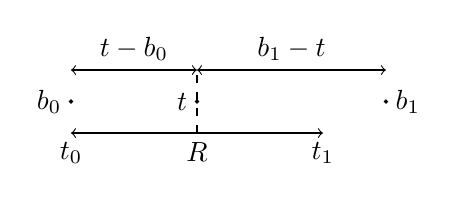
\begin{tikzpicture}[scale=2]
    \coordinate (A) at (-1,0);
    \coordinate (B) at (-0.2,0) ;
    \coordinate (C) at (1,0) ;
    \node[left] at (A) {$b_{0}$};
    \node[left] at (B) {$t$};
    \draw[dashed] ([yshift = -2mm]B) -- ([yshift = 2mm]B);
    \node[right] at (C) { $b_{1}$};
    \draw[fill=black] (A) circle (0.01);
    \draw[fill=black] (B) circle (0.01);
    \draw[fill=black] (C) circle (0.01);
    \draw[<->] ([yshift = 2mm]A) --  ([yshift = 2mm]B) node[above,midway] {$t-b_{0}$};
    \draw[<->] ([yshift = 2mm]B) --  ([yshift = 2mm]C) node[above,midway] {$b_{1}-t$};
    \draw[<->] (-1,-0.2)node[below]{$t_{0}$} --  (0.6,-0.2)node[below]{$t_{1}$} node[below,midway] {$R$};
\end{tikzpicture}


\end{document}